\documentclass{article}
\usepackage{graphicx}

\title{About a Feline Ambassador}
\author{
	Zayd Hammoudeh \\
	San Jose State University \\
	zayd.hammoudeh@sjsu.edu
}

\begin{document}
\maketitle


\section{Personal History}
I do not usually talk about myself, but when I do, I talk about my cat.\\

In April 2010, the American economy was gripped by its most severe economic crisis in at least a generation.  There was in a deep recession.  It was in this climate that a great savior was born; her name is Muffins.  

\begin{figure}[ht!]
\centering
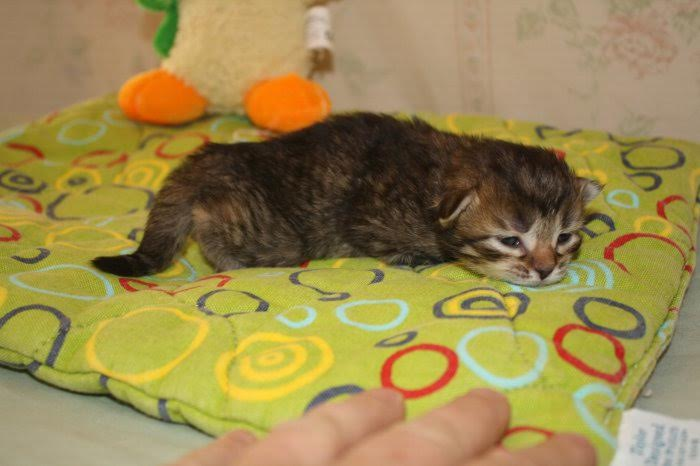
\includegraphics[width=90mm]{./images/muffins.jpg}
\caption{A Week Old Muffins}
\end{figure}

She is the first cat I have ever owned.  She is a purebred Siberian.  Her interests include: sleeping, eating tuna fish, and looking out the window.\\

The reason I chose to get a Siberian cat is because they are purported (perhaps dubiously) to be hypoallergenic. They are also a very healthy breed as they were more recently domesticated.  I had fears concerning the effects of a feline on my allergies as I had some previous negative experiences.  In the first years I have owned her, she has been a pure pleasure to be around.

\section{Career Goals}
I am impressed by the ground working done by the renowned dog rehabilitator Cesar Millan, host of the critically acclaimed television show "Dog Whisperer." It is my hope that I could have an equally successful television program which I will entail "Cat Telepathist"  where I will rehabilitate troubled and stray cats through the power of extrasensory perception (ESP).\\

If my "Cat Telepathist" show were not to find a niche with audiences, my second television show is modeled after the former television show "Crossing Over with John Edward." \cite{calderwood} I plan to call the show "You have Cat to be Kitten Me with Zayd Hammoudeh" and will be used to give grieving families the opportunity to communicate with their deceased feline family members.

\section{Research Interests}

My research interests are varied, but as part of my future career in inter-species psychic connections, I am a regular reader of the work of Sonya Fitzpatrick who is "widely regarded as the most experienced and trusted animal communicator in the world." \cite{fitzpatrick_2013}  Her best books are \underline{Cat Talk} \cite{fitzpatrick2003cat} and \underline{What the Animals Tell Me} \cite{fitzpatrick_smith_1997}.


\bibliographystyle{plain}
\bibliography{zayd_hammoudeh_biblio}

\end{document}